% THIS IS SIGPROC-SP.TEX - VERSION 3.1
% WORKS WITH V3.2SP OF ACM_PROC_ARTICLE-SP.CLS
% APRIL 2009
%
% ----------------------------------------------------------------------------------------------------------------
% This .tex file (and associated .cls V3.2SP) *DOES NOT* produce:
%       1) The Permission Statement
%       2) The Conference (location) Info information
%       3) The Copyright Line with ACM data
%       4) Page numbering
% ---------------------------------------------------------------------------------------------------------------
% For tracking purposes - this is V3.1SP - APRIL 2009

\documentclass{acm_proc_article-sp}
\usepackage{graphicx}


\begin{document}

\title{Copy and Paste Habits and Improvements for the Everyday Programmer}
\subtitle{February 1 Deliverable}

\numberofauthors{4} 
\author{
\alignauthor
Brian Clee\\
       %\affaddr{NC State University}\\
       %\affaddr{Address One}\\
       \email{bpclee@ncsu.edu}
\alignauthor
Effat Farhana\\
       %\affaddr{NC State University}\\
       %\affaddr{Address Two}\\
       \email{efarhan@ncsu.edu}
\and % go to new row
\alignauthor
Arjun Madan\\
       %\affaddr{NC State University}\\
       %\affaddr{Address Three}\\
       \email{amadan2@ncsu.edu}
\alignauthor
Ran Tan\\
       %\affaddr{NC State University}\\
       %\affaddr{Address Four}\\
       \email{rtan2@ncsu.edu}
}

\date{1 February 2016}


\maketitle
\begin{abstract}
Abstract text. 
\end{abstract}

%see http://www.acm.org/sigs/publications/sigguide-v2.2sp section 2.3.2
% A category with the (minimum) three required fields
\category{D.2.2}{Software Engineering}{Design Tools and Techniques}[Modules and interfaces, programmer workbench, user interfaces]
%A category including the fourth, optional field follows...
\category{D.2.3}{Software Engineering}{Coding Tools and Techniques}[Program Editors]

% see http://www.acm.org/sigs/publications/sigguide-v2.2sp section 2.3.3
\terms{Human Factors, Management, Performance, Theory}

\keywords{Code cloning, code duplication, copy and pasting, eclipse plug-ins, programmer habits, programmer productivity}

\section{Introduction}
One of the most common operations computer users apply in their daily computer use is copy and paste. An incredibly simple to understand tool, copy and paste allows users to take information from one location, briefly store it, and then leave that information elsewhere. This simple tool is commonplace for computer users, and it is especially useful to computer programmers. 

In the field of computer programming users frequently make use of the copy and past operation for a myriad of reasons. For one, it is essential in the practice of relocating, regrouping, or reorganizing code from one place to another. Along these lines programmers also use the command in the act of reordering parts of their code, rather than rewriting. Finally, perhaps the most common use of the copy and paste command is when a programmer copies a block of code, either from inside sources within their existing code base or outside it, to use as a structural template ~\cite{ooplCP}.

However, while there is much to be gained from the copy and paste operation for programmers, it is also important to realize that despite the operation's convenience and simplicity, the act of copying and pasting introduces a variety of errors. In one study analyzing programmer habits, it was found that copying and pasting can introduce errors by pasting incomplete copies, and failing to update their context. In this study they found that these sorts of errors actually reduced productivity as a whole for the programmer by delaying development in the long run ~\cite{maintenenceStudy}

Yet despite the apparent errors that can be introduced by copying and pasting, programmers still make use of the operation in their core work-flow. In another study done it was found that on average every programmer copy and pastes 16 times while programming ~\cite{ooplCP}. Clearly this command has become part of programming vernacular despite the problems it can cause.

In this paper we investigate the copy and paste command as used in software engineering in greater detail. In particular we present a literature review on the topic as it has been investigated in numerous studies and research experiments. We look at the user patterns and behavioral components that go into using this command, as well as the command itself in practice. We also look at heavier theoretical applications to copying and pasting such as code cloning and pattern detection. Ultimately though, we use this research to show that there is untapped potential in the copy and paste command for programmers, which can be addressed by a fully featured clipboard manager plug-in for the Eclipse IDE, similar to one described in ~\cite{ooplCP}.

\section{Project Goals}
Effat!
PUTG
Project features
\\
1. Multi-item\\
 User often switches back and forth between windows to copy and paste. If we can design a clipboard that holds \textit{ multiple item at a time}, it can reduce switching. For example, if a user copies a students name, email address, institution name to a form, a multi- item clipboard manager can hold each item separately and paste it altogether. \\
 
 Multiple item can also be from multiple windows. Figure \ref{fig:Multi} describes two different variations of multiple item copy pasting ~\cite{cpHabits}. The upper portion is copying multiple items from a single source. The bottom portion depicts copying from multiple windows.\\
 
 The proposed method for copying multiple items from a single source has already been described above. For multiple items from different windows, the copied item from all the sources will be pasted to destination at a time, and each copied item from one window  will move to the next window via clipboard.\\
 \begin{figure}[h]
 \centering
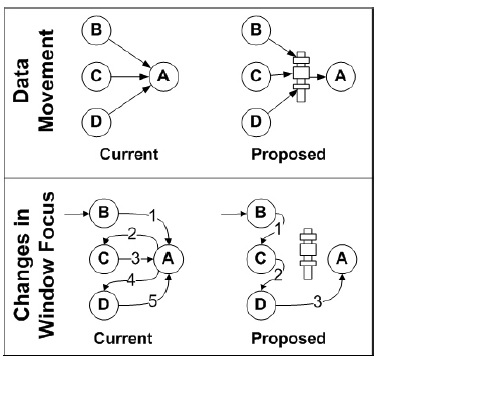
\includegraphics[width=10cm]{MultiItem}
\caption{Multiple Item Copy and Pasting}
    \label{fig:Multi}
\end{figure}
2. System Wide copy\\
For this purpose, we perform a finer level of analysis and consider user copy and paste behavior between windows, where an application may have multiple windows (e.g., worksheets in spreadsheets, tabs in browsers,  find dialog for a word processor). A graphical representation of system wise copy and pasting is illustrated in Figure \ref{fig:System} ~\cite{cpHabits}. Advanced window management techniques such as restacking or rolling partially overlapping windows have been shown to be effective ~\cite{overlapWindow}. Adding a feature to reduce the overhead of switching among multiple windows would be desirable.
 \begin{figure}[h]
 \centering
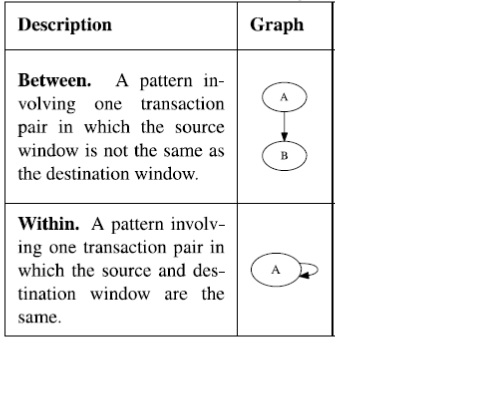
\includegraphics[width=10cm]{Window}
\caption{System Wide Copy and Pasting}
    \label{fig:System}
\end{figure}
3. Context Awareness\\
    a. How do we display items?\\
    b. How do we order the items?\\
4. Code Cloning   \\
5. Design Pattern detection\\ 
6. Touch screen interactions\\

\section{User Patterns and Behavior}
Brian!
Why do we need to copy/paste
Studies that show we copy/paste a lot

\section{Copy and Paste in Practice}
Arjun!
Default clipboard, between windows, studies on copy and pasting with stats, current existing solutions.

All operating systems come with a system clipboard. It involves storing a single item, whether a piece of text, URL, image, or file to a place in memory. This item can then be retrieved multiple times and copied to appropriate locations. The main drawback of such a system is that when a new item is copied to memory, all information regarding the previous one is lost. If users wanted to obtain this information again, they would have to find the item and copy or cut it again. Programmers typically use the  clipboard to copy and paste code from other sources into the code they're writing.~\cite{codeReuse}

There are many solutions that exist that make the system clipboard easier and quicker to use. X Window~\cite{overlapWindow} is an application that speeds up by having users drag to select text and then use the middle-click of the mouse to paste, instead of the default keyboard option. While this does offer more convenience, and saves some time, it doesn't address the main pain point with the system clipboard.

A significant improvement over this is the multi-item clipboard.~\cite{cpHabits} It stores multiple items in memory, and allows a way of retrieving them through shortcuts or a visual interface. The main advantage of this method is the time users save, as they don't have to go back to the source of an older item in order to paste it. Figure 1 shows how there are fewer changes in window focus, thereby saving the user time. A study conducted shows that this is actually the most common method of copy and pasting, resulting in the time saved by having a multi-item clipboard being significant.

These type of multi-clipboards can be especially useful for programmers where studies show that an average programmer copies and pastes code 16 times for every hour of programming.~\cite{ooplCP} A problem with the existing solutions is that they are not targeted specifically at programmers. A clipboard manager could help eliminate some of the common problems a programmer faces. 


\section{Code Cloning and Pattern Detection}
Ran!
Theoretical section on code cloning and pattern detection and management.
\iffalse
Our study of copy and paste in IDE environment falls into the general area of code clone. A study of the concepts and techniques of code clone will be of great support for our project. 
\fi
The concept of clones.
According to Ira Baxter, “Clones are segments of code that are similar according to some definition of similarity.”

The causes of clones.

The consequences of clones.

The evolvement of clones.





\section{Conclusion}
Arjun!
Refresh on our main points and themes. Talk about our 3/4 features we will be doing.

\bibliographystyle{abbrv}
\bibliography{citations}

%\balancecolumns 

\end{document}
